%\chapter[Formulation du problème de propagation d'interfaces $\contgeom{1}$ \piecewise\ en \troisD]{Formulation mathématique du problème de propagation d'interfaces régulières \piecewise\ en trois dimensions}
\chapter[Formulation du problème de propagation d'interfaces $\contgeom{1}$ \piecewise]{Formulation mathématique du problème de propagation d'interfaces régulières \piecewise\ en trois dimensions}
\chaptermark{Formulation du problème de propagation d'interfaces $\contgeom{1}$ \piecewise}%\ en \troisD}
\label{chap:formulation_probleme_propagation}

Ce premier chapitre a pour objectif de formaliser le problème central de la thèse : la propagation d'interfaces régulières \piecewise\ en trois dimensions. 
Pour cela, on rappelle dans un premier temps les éléments de la géométrie différentielle des courbes et surfaces auxquels on aura recours tout au long du manuscrit.
On accorde un intérêt particulier aux surfaces de régularité $\contgeom{1}$ \piecewise, ainsi qu'à leur description par décomposition cellulaire via la représentation par les frontières.
On donne ensuite la formulation lagrangienne traditionnelle du problème de propagation d'interface et met en évidence ses limites dans le contexte de la thèse.
On conclut ce chapitre en introduisant une formulation plus adéquate du problème, basée sur le principe de Huygens.



\section{Description et représentation des surfaces régulières \piecewise}
[décomposition en nappes régulières ($\contgeom{1}$), courbes singulières (crêtes?) et points irréguliers (coins?) (\cf notes Huygens)]
\par\bigskip
(Inspiré par \cite[p.65]{rossignac1985} et \cite[Section 2.6]{rossignac1986}.)\par

\subsection{Géométrie différentielle des (courbes et) surfaces}
%[courbes et surfaces paramétriques : vocabulaire (arc, carreau, espace et domaine paramétriques, carreau restreint, courbes de restriction), vecteur(s) et plan tangents, vecteur (pseudo-)normal, notion de continuités paramétrique/géométrique, tenseur métrique, première et seconde formes fondamentales, courbures principales, gaussienne et moyenne]
%\par\bigskip
%Dans ce manuscrit, on appelle \textit{carreau de surface paramétrique} de classe $\contdiff{k}$ tout couple $(\uvdomain, \bs)$ où $\uvdomain \subset \reals^2$, $\bs : \uvdomain \to \reals^3$ est une fonction de classe $\contdiff{k}$ sur $\uvdomain$, et $k \in \integers$. 
%On appelle $\uvdomain$ le \textit{domaine paramétrique} d'un tel carreau et on dit que $\bs$ en est une \textit{paramétrisation}. 
%Par commodité, on désignera parfois le carreau simplement par $\bs$.
%\par
%Le support $\bs(\uvdomain)$ 
notion de continuité géométrique : point régulier/singulier $\to$ notion de plan tangent\\
paramétrisation (locale), atlas, continuité paramétrique

\begin{figure}
	\centering
	\setlength{\imagewidth}{80mm}%
\setlength{\imageheight}{\imagewidth}%
\DTLsetseparator{,}%
\DTLloaddb[noheader,keys={x,y,a}]{dbcorners}{figures/data/piecewise_smooth_surface/corners_xya.dat}%
\DTLloaddb[noheader,keys={x,y,a}]{dbedgemidp}{figures/data/piecewise_smooth_surface/edge_midpoints_xya.dat}%
\begin{tikzpicture}[%
		x=\imagewidth, y=\imageheight,
		img/.style={anchor=south west, inner sep=0},
		anot/.style={-{Latex[length=4pt]}, shorten >=2pt},
		anotpoint/.style={anot, shorten >=5pt},
	]
	%%% SURFACE
	\node[img] at (0,0) {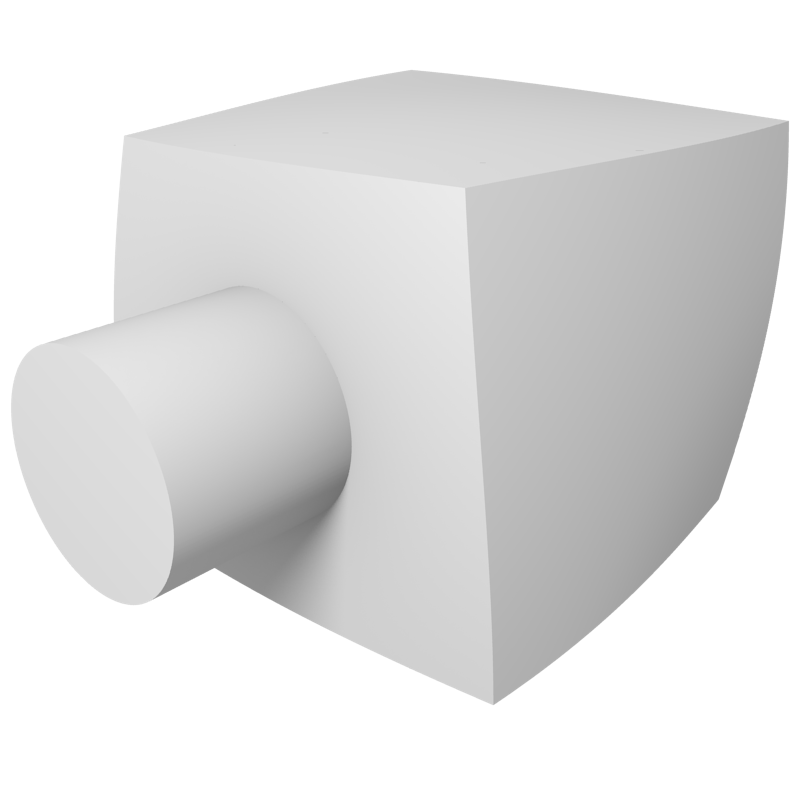
\includegraphics[width=\imagewidth]{piecewise_smooth_surface/surface}};
	%%% HIDDEN EDGES
	\node[img] at (0,0) {
\includegraphics[width=\imagewidth]{piecewise_smooth_surface/edges_hidden}};
	%%% HIDDEN CORNERS
	\DTLforeach*{dbcorners}{\locx=x, \locy=y, \loca=a}{%
		\ifnum \loca = 0
			\fill[black] (\locx,\locy) circle (1.0pt);
		\fi
	}%
	%%% SURFACE (semi-transparent to mask hidden edges & corners)
	{\transparent{0.75}
		\node[img] at (0,0) {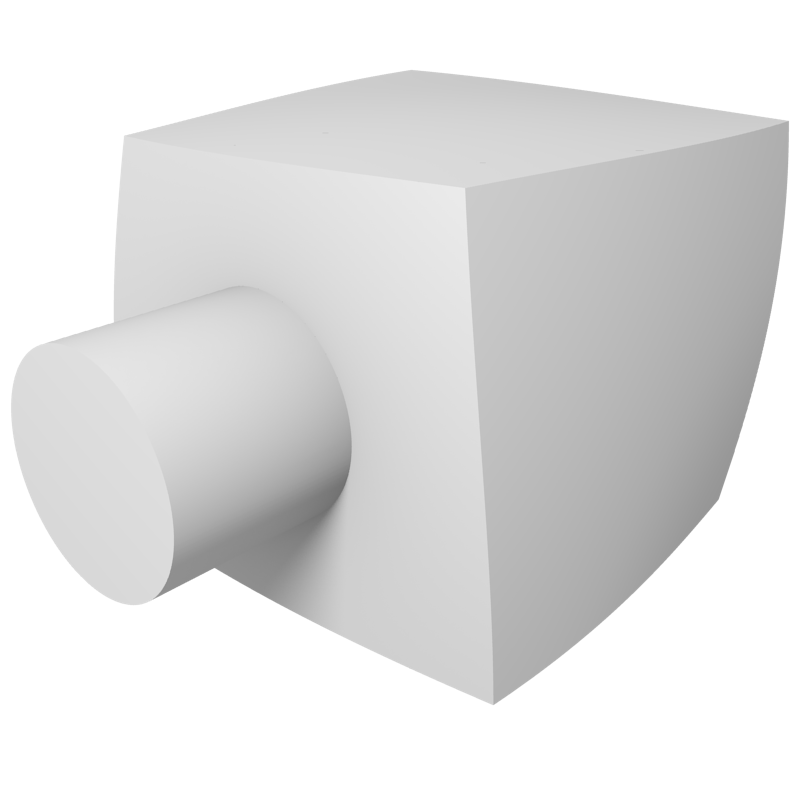
\includegraphics[width=\imagewidth]{piecewise_smooth_surface/surface}};
	}%
	%%% VISIBLE EDGES
	\node[img] at (0,0) {
\includegraphics[width=\imagewidth]{piecewise_smooth_surface/edges_visible}};
	%%% VISIBLE CORNERS
	\DTLforeach*{dbcorners}{\locx=x, \locy=y, \loca=a}{%
		\ifnum \loca = 1
			\fill[black] (\locx,\locy) circle (1.2pt);
		\fi
	}%
	%
	%%% ANOTATIONS
	\DTLassign{dbcorners}{6}{\locxa=x,\locya=y,\loca=a}% 	
	\DTLassign{dbcorners}{4}{\locxb=x,\locyb=y,\loca=a}% 
	\DTLassign{dbcorners}{1}{\locxc=x,\locyc=y,\loca=a}% 
	%\node[anchor=west] (anotSingPts) at (\locxb,{0.5*(\locya + \locyb)}) {points singuliers};
	\node[anchor=east] (anotSingPts) at (1.2,0.2) {coins};
	\draw[anot] (anotSingPts) to [bend left=10] (\locxa, \locya);
	\draw[anot] (anotSingPts) to [bend right=20] (\locxb, \locyb);
	\draw[anot] (anotSingPts) to [bend right=10] (\locxc, \locyc);
	%
	\DTLassign{dbedgemidp}{19}{\locxa=x,\locya=y,\loca=a}% 	
	\DTLassign{dbedgemidp}{7}{\locxb=x,\locyb=y,\loca=a}% 
	\DTLassign{dbedgemidp}{14}{\locxc=x,\locyc=y,\loca=a}% 
	\node[anchor=west] (anotSingCurv) at (-0.2,0.9) {crêtes};
	\draw[anot] (anotSingCurv) to [bend right=10] (\locxa, \locya);
	\draw[anot] (anotSingCurv) to [bend right=40] (\locxb, \locyb);
	\draw[anot] (anotSingCurv.east) to [bend left=10] (\locxc, \locyc);
\end{tikzpicture}
\DTLgdeletedb{dbcorners}%
\DTLgdeletedb{dbedgemidp}%

	\caption{Surface régulière \piecewise\ dont les courbes et points singuliers sont mis en évidence.}
	\label{fig:piecewise_smooth_surface_decomposition}
\end{figure}

%La frontière $\boundary{\Omega}$ du solide $\Omega$ est une surface de continuité $\contgeom{1}$ (\ie possède une direction normale continue) \piecewise. 
%Les singularités géométriques de $\boundary{\Omega}$ peuvent être de dimension 1 (courbes) ou 0 (points).
%Les courbes singulières de $\boundary{\Omega}$ sont elle-mêmes des variétés différentielles de continuité $\contgeom{1}$ (\ie possède une direction tangente continue) excepté aux points singuliers.

\subsection{Représentation par les frontières (\brep)}
Origine, utilisation, concept, définitions formelles des entités, lien avec la décomposition d'une surface $\contgeom{1}$ \piecewise, (géométrie différentielle des courbes et surfaces paramétriques), structures de données (DCEL)

\begin{enumerate}
	\item l'ensemble des points singuliers est un sous-ensemble des sommets \brep
	\item l'ensemble des courbes singulières est un sous-ensemble des arêtes \brep
%	\item chaque arête \brep\ vive est contenue dans une courbe singulière
\end{enumerate}

\begin{figure}
	\centering
	\colorlet{topo_color}{mycolor_5}
\colorlet{orient_color}{topo_color!60!mycolor_2}
\colorlet{group_color}{topo_color!40!mycolor_3}
\colorlet{geom_color}{mycolor_1}%{mycolor_3}
\def\bigsep{5mm}
\def\smallsep{2.5mm}
\pgfdeclarelayer{bg}    % declare background layer
\pgfsetlayers{bg,main}  % set the order of the layers (main is the standard layer)
\begin{tikzpicture}[
	x = 30mm,
	y = 9.75mm,
	arrow/.style={thick, -stealth', shorten <= 2pt, shorten >= 2pt},
	bounded/.style={arrow, dash pattern=on 4pt off 2pt},
	described/.style={arrow},
	composed/.style={arrow, dash pattern=on 1.5pt off 1.5pt},
	box/.style={rectangle, rounded corners=0.8ex},
	number/.style={font=\footnotesize},
	topo/.style={fill=topo_color!33!white},
	geom/.style={fill=geom_color!33!white},
	orient/.style={fill=orient_color!33!white},
	group/.style={fill=group_color!33!white},
	type/.style={font=\bfseries},%, anchor=east},
	label/.style={anchor=west, inner sep=2pt, font=\scriptsize},
	class/.style={dotted, thick, line cap=round},
	bigclass/.style={class, rounded corners=\bigsep, dash pattern=on 0.8pt off 3.2pt},
	smallclass/.style={class, rounded corners=\smallsep, dash pattern=on 0.3pt off 2.8pt},
	]
	% entités topologiques
	\node[box, topo] at (-1,1) (volume) {Solide};
	\node[box, topo] at (0,1) (face) {Face};
	\node[box, topo] at (1,1) (edge) {Arête};
	\node[box, topo] at (2,1) (vertex) {Sommet};
	% entités de groupement
	\node[box, group] at (-1,3) (shell) {Coquille};
	\node[box, group] at (0,3) (wire) {Contour};
	% entités d'orientation
	\node[box, orient] at (1,3) (halfedge) {Co-arête};
	% entités géométriques
	\node[box, geom] at (0,-1) (surface) {Surface};
	\node[box, geom] at (1,-1) (curve) {Courbe};
	\node[box, geom] at (2,-1) (point) {Point};
	%
	% relations "décrit par"
	\draw[described] (face) -- (surface);
	\draw[described] (edge) -- (curve);
	\draw[described] (vertex) -- (point);
	% relations "délimité par"
	\draw[bounded] (volume) -- 
		node[number,left]{$1+n_{\mathrm{s}}^{\mathrm{int}}$} 
		(shell);
	\draw[bounded] (face) -- 
		node[number,right]{$1+n_{\mathrm{w}}^{\mathrm{int}}$} 
		(wire);
	\draw[bounded] (edge) -- node[number,above]{$2$} (vertex);
	% relations "composé de"
	\draw[composed] (shell) -- node[number,above right]{$n$} (face);
	\draw[composed] (wire) -- node[number,above]{$n$} (halfedge);
	\draw[composed] (edge) -- node[number,right]{$2$} (halfedge);
	%
	% noms de classes
	\gettikzxy{(current bounding box.east)}{\xbbE}{\ybbE}%
	\node[type, geom_color!90!gray] (geomet) at (-1,-1) {Géométrie};
	\node[type, anchor=east, orient_color!90!gray] (orientation) at ({\xbbE-0.5*\smallsep},3) {Orientation};
	\gettikzxy{(halfedge.east)}{\xhE}{\yhE}%
	\gettikzxy{(orientation.west)}{\xoW}{\yoW}%
	\gettikzxy{(shell.west)}{\xsW}{\ysW}%
	\node[type, anchor=east, group_color!90!gray] (grouping) at ({\xsW-\xoW+\xhE},3) {Groupement};
	\gettikzxy{(grouping.west)}{\xgrW}{\ygrW}%
	\gettikzxy{(grouping.south)}{\xgrS}{\ygrS}%
	\gettikzxy{(volume.south)}{\xvS}{\yvS}%
	\node[type, anchor=west, topo_color!90!gray] (topology) at (\xgrW,{0.5*(\ygrS-\smallsep + \yvS-\bigsep)}) {Topologie};
	%
	% classes
	\gettikzxy{(vertex.south east)}{\xtSE}{\ytSE}%
	\gettikzxy{(shell.north)}{\xtN}{\ytN}%
	\gettikzxy{(grouping.west)}{\xtW}{\ytW}%
	\gettikzxy{(geomet.west)}{\xgeW}{\ygeW}%
	\gettikzxy{(topology.north)}{\xtM}{\tmp}%
	\gettikzxy{(grouping.south)}{\tmp}{\ytM}%
	\gettikzxy{(halfedge.south west)}{\xoSW}{\yoSW}%
	\gettikzxy{(halfedge.north)}{\xoN}{\yoN}%
	\gettikzxy{(orientation.north east)}{\xoNE}{\yoNE}%
	\gettikzxy{(grouping.south west)}{\xgrSW}{\ygrSW}%
	\gettikzxy{(wire.south)}{\xgrS}{\ygrS}%
	\gettikzxy{(wire.north east)}{\xgrNE}{\ygrNE}%
	\gettikzxy{(surface.south)}{\xgeS}{\ygeS}%
	\gettikzxy{(surface.north)}{\xgeN}{\ygeN}%
	\begin{pgfonlayer}{bg}    % select the background layer
		\draw[bigclass, topo_color, fill=topo_color!8!white] 
		({\xtSE+\bigsep},{\ytSE-\bigsep}) --
		({\xtSE+\bigsep},{\ytN+\bigsep}) --
		({\xtW-\bigsep},{\ytN+\bigsep}) --
		({\xtW-\bigsep},{\ytSE-\bigsep}) -- cycle;
		%
		\draw[smallclass, orient_color, fill=orient_color!8!white] 
		({\xoSW-\smallsep},{\yoSW-\smallsep}) -- 
		({\xoNE+\smallsep},{\yoSW-\smallsep}) -- 
		({\xoNE+\smallsep},{\yoN+\smallsep}) -- 
		({\xoSW -\smallsep},{\yoN+\smallsep}) -- cycle;
		%
		\draw[smallclass, group_color, fill=group_color!8!white] 
		({\xgrSW-\smallsep},{\ygrS-\smallsep}) -- 
		({\xgrNE+\smallsep},{\ygrS-\smallsep}) -- 
		({\xgrNE+\smallsep},{\ygrNE+\smallsep}) -- 
		({\xgrSW -\smallsep},{\ygrNE+\smallsep}) -- cycle;
		%
		\draw[bigclass, geom_color, fill=geom_color!8!white]
		({\xgeW-\bigsep},{\ygeS-\bigsep}) -- 
		({\xtSE+\bigsep},{\ygeS-\bigsep}) -- 
		({\xtSE+\bigsep},{\ygeN+\bigsep}) -- 
		({\xgeW-\bigsep},{\ygeN+\bigsep}) -- cycle;
	\end{pgfonlayer}
	% légende des relations
	\coordinate (lgd) at ({\xtW-\bigsep+2pt},{0.5*(\ygeS+\ygeN)});
	\foreach \i in {0,1,2}{
		\coordinate (L\i) at ([yshift={-(\i-1)*2.8ex}]lgd);
		\coordinate (R\i) at ([xshift=7.5mm]L\i);
	}
	\draw[described] (L0) -- (R0) node[label] (lbl0) {décrit par};
	\draw[bounded]   (L1) -- (R1) node[label] (lbl1) {délimité par};
	\draw[composed]  (L2) -- (R2) node[label] (lbl2) {composé de};
	\node[draw=black!25,
	inner sep=2pt,
	rounded corners=\smallsep,
	fit={(L0) (lbl0) (lbl1) (lbl2)}] {};
\end{tikzpicture}
	\caption{Hiérarchie des éléments constituant un modèle \brep.}
	\label{fig:BRep_hierarchy}
\end{figure}



\begin{figure}
	\centering
	\setlength{\imagewidth}{80mm}%
\setlength{\imageheight}{\imagewidth}%
\DTLsetseparator{,}%
\DTLloaddb[noheader,keys={x,y,a}]{dbverts}{figures/data/BRep/verts_xya.dat}%
\begin{tikzpicture}[%
	x=\imagewidth, y=\imageheight,
	img/.style={anchor=south west, inner sep=0}]
	%%%%%%%%%%%%%%%% SHELL %%%%%%%%%%%%%%%%
	%%% FACES
	\node[img] at (0,0) {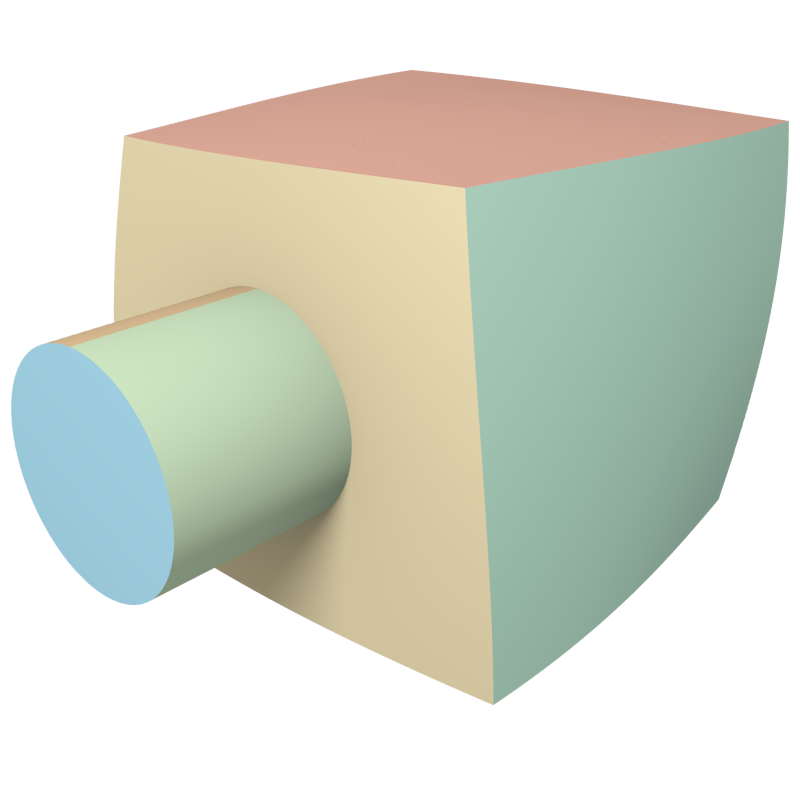
\includegraphics[width=\imagewidth]{BRep/shell}};
	%%% HIDDEN EDGES
	\node[img] at (0,0) {
\includegraphics[width=\imagewidth]{BRep/edges_hidden}};
	%%% HIDDEN VERTICES
	\DTLforeach*{dbverts}{\locx=x, \locy=y, \loca=a}{%
		\ifnum \loca = 0
			\fill[black] (\locx,\locy) circle (1.0pt);
		\fi
	}%
	%%% FACES (semi-transparent to mask hidden edges & verts)
	{\transparent{0.75}
		\node[img] at (0,0) {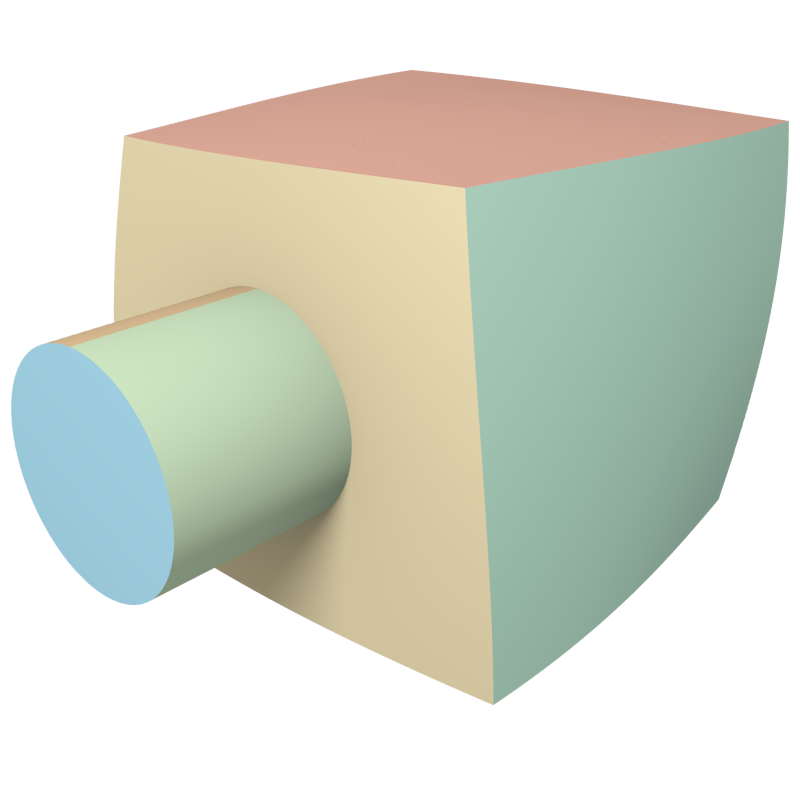
\includegraphics[width=\imagewidth]{BRep/shell}};
	}%
	%%% VISIBLE EDGES
	\node[img] at (0,0) {
\includegraphics[width=\imagewidth]{BRep/edges_visible}};
	%%% VISIBLE VERTICES
	\DTLforeach*{dbverts}{\locx=x, \locy=y, \loca=a}{%
		\ifnum \loca = 1
			\fill[black] (\locx,\locy) circle (1.0pt);
		\fi
	}%
\end{tikzpicture}
\DTLgdeletedb{dbverts}%
%%%%%%%%%%%%%%%%%%%%%%%%%%%%%%%%%%%%%%
%
%%%%%%%%%%%%%%%% FACES %%%%%%%%%%%%%%%%
\def\imfacew{44mm}
\def\ngriduv{6}
\def\vertsep{0.05}
\def\edglabsepuv{0.17}
\def\wirlabsepuv{0.18}
\def\edglabsepxyz{0.06}
\def\iniwclr{0.3}
\def\decwclr{0.3}%{0.2}
\def\uvscale{0.34}
\def\uvyshift{-0.7}
\pgfmathsetmacro\sepyshift{0.5 * (\uvyshift+\uvscale)}%
%
\begin{tikzpicture}[%
	x = \imfacew, y = \imfacew,
	gridtick/.style={red, fill=white, font=\tiny, inner sep=0.5pt},
	img/.style={anchor=south west, inner sep=0},
	label/.style={inner sep=1pt, font=\scriptsize},
	uvgrid/.style={black!10!white},
	curv/.style={line width=0.8pt, line cap=round},
	spacelabel/.style={anchor=north, rotate=90, inner sep=0, font=\bfseries},
	]
	\foreach \jfa/\ifa in {-1/007, 0/008, 1/002}{%
		\figbrepface{\ifa}{{1.05*\jfa - 0.5}}{{-\sepyshift}}%\hfill
	}%
	\draw[very thick, gray, dashed] 
	({-0.5*\textwidth},0) -- ++ 
	(\textwidth,0);
	\node[spacelabel] (xyzspace) at 
	({-0.5*\textwidth},{-\sepyshift+0.5}) {Espace euclidien\vphantom{Espace paramétrique}};
	\node[spacelabel] (uvspace) at 
	({-0.5*\textwidth},{\sepyshift-\uvscale}) {Espace paramétrique\vphantom{Espace euclidien}};
\end{tikzpicture}

	\caption{Modèle \brep\ d'une surface régulière par morceaux.}
	\label{fig:BRep}
\end{figure}



\section{Formulation lagrangienne du problème de propagation d'interface}
On considère une interface $\Sigma$ entre deux milieux distincts (\eg un solide et un fluide).
Dans cette thèse, on se concentre sur des problèmes en trois dimensions. 
$\Sigma$ représente donc une surface (\ie une variété de dimension 2) que l’on supposera orientable et fermée (\ie sans bord).
De cette manière, l'interface sépare un domaine \textit{intérieur} $\Omega$ --- que l'on supposera ouvert --- et un domaine \textit{extérieur} $\complement{\Omega} = \reals^3 \setminus \Omega$.
\par
%[EDP avec vecteur vitesse ou vitesse normale, problème de définition au niveau des courbes singulières et points irréguliers]
%\par\bigskip
Le problème que l'on cherche à résoudre consiste à déterminer l’évolution au cours du temps de l'interface $\Sigma$ étant données sa position actuelle ainsi que sa vitesse de propagation.
Dans la formulation lagrangienne traditionnelle, ce problème est exprimé sous la forme d'une équation aux dérivées partielles (EDP) pour le vecteur position $\bx$ d'un point de l'interface.
L'équation décrivant la propagation suivant un champ de vecteur vitesse $\vrm{u} : \Sigma \times \reals \to \reals^3$ est
\begin{equation}
	\frac{\partial \bx}{\partial t} = \vrm{u}(\bx,t).
	\label{eq:lagrange_vecteur_vitesse}
\end{equation}
On peut également considérer que chaque point de $\Sigma$ se déplace le long de la direction normale à l'interface suivant un champ de vitesse normale $\nu : \Sigma \times \reals \to \reals$. 
L'équation décrivant la propagation est alors
\begin{equation}
	\frac{\partial \bx}{\partial t} = \nu(\bx,t) \unv(\bx,t).
	\label{eq:lagrange_vitesse_normale}
\end{equation}
En principe, les formulations \eqref{eq:lagrange_vecteur_vitesse} et \eqref{eq:lagrange_vitesse_normale} sont équivalentes puisque la composante tangentielle du vecteur vitesse n'affecte pas la forme de l'interface. 
\par\bigskip
La formulation lagrangienne ne permet d'obtenir une solution au problème de propagation d'interface que dans le cas où cette dernière est \textit{globalement} régulière et le reste tout au long de sa propagation. 
En effet, puisque la direction normale $\unv$ n'est pas définie au niveau des courbes et points singuliers de $\Sigma$, le déplacement de ces points est ambigu. 
On peut notamment distinguer deux cas \cite{jiao2007}.
\par
Premièrement, si l'interface subit un mouvement d'advection (comme le transport d'un fluide ou encore la déformation d'un solide sous l'effet de contraintes mécaniques) alors ses singularités géométriques sont préservées au cours de la propagation.
\par
En revanche, si l'interface se propage à la manière d'un front d'onde (comme la progression d'une flamme, d'un dépôt de matière ou encore l'ablation d'un solide) alors les singularités sont soit préservées soit régularisées, suivant la convexité locale de l'interface.
C'est essentiellement sur ce deuxième type de propagation que la thèse se concentre.
\par\bigskip
Puisque l'on s'intéresse ici à la propagation d'interfaces régulières seulement \piecewise, il est nécessaire d'obtenir une meilleure formulation du problème qui s'affranchisse des ambiguïtés ainsi mises en évidence. 
Plutôt que de poser le problème sous la forme d'une équation différentielle, cette nouvelle formulation se présente sous la forme d'une construction géométrique.

\section{Principe de Huygens avec condition d'entropie}
\label{section:principe_huygens}
\def\p{\vit{p}}
\def\q{\vit{q}}
%
%[Histoire, formulation, notion d'enveloppe de sphères/boules, construction géométrique au lieu de EDP, équations définissant l'EdS propre à 1/2 paramètre(s), différence d'ordre 2 avec transport suivant la normale, définitions implicites (\cf notes Huygens)]
%\par\bigskip
Alors qu'il développait un modèle ondulatoire de la propagation de la lumière, Christiaan Huygens proposa le principe suivant : chaque point de l'espace atteint par une onde lumineuse se comporte comme la source d'une ondelette secondaire émise dans toutes les directions. 
Si le milieu de propagation est homogène et isotrope alors les ondelettes sont sphériques. 
Le front d'onde, qui se propage ainsi de proche en proche, est alors formé par l'\textit{enveloppe} de ces ondelettes, \ie la surface qui est tangente à chacune d'elles et dont chaque point est un point de tangence avec une ondelette.
\par
Le principe de Huygens permet de décrire de nombreux phénomènes analogues à la propagation d'une onde dans un milieu tels que la progression d'une flamme. 
\textit{(développer \ldots)}

\par\bigskip
\begin{enumerate}
	\item distinguer propagation d'une onde et d'une interface entre deux milieux matériels $\to$ condition d'entropie
	\item l'une peut s'auto-intersection, l'autre non
	\item formaliser la notion d'enveloppe des sphères $\EoS{\Sigma}{\rho}$ (surface tangente à toutes les sphères et en tout point tangente à une sphère) $\to$ système d'équations avec $\implicitsphere_{\rho} : (\bx,\p) \mapsto \normtwo{\bx - \p}^2 - \rho^2(\p)$
	\item formaliser la notion d'enveloppe des boules $\EoB{\Sigma}{\rho} := \boundary{\left\{\Omega \cup \sphere[\Sigma][\rho]\right\}}$
	\item (donner définition implicite de $\EoB{\Sigma}{\rho}$)
	\item à condition que $\rho$ soit suffisamment régulière (continuité à déterminer), $\EoB{\Sigma}{\rho} \subset \EoS{\Sigma}{\rho}$
\end{enumerate}


%Dans la suite, étant donné un sous-ensemble (ouvert ou fermé) $E$ de $\reals^d$, on notera $\complement{E} := \reals^d \setminus E$ son \textit{complémentaire}, $\boundary{E}$ sa \textit{frontière}, $\interior{E}$ son \textit{intérieur} et $\closure{E} = E \cup \boundary{E}$ son \textit{adhérence}.
%\par\bigskip
%
%\def\p{\vit{p}}
%\def\q{\vit{q}}
%Soient $r> 0$ et $\p$ un point de $\reals^3$. 
%On note $\sphere[\p][r]$ la sphère de rayon $r$ centrée en $\p$
%\begin{equation}
%    \sphere[\p][r] := \left\{ 
%        \bx \in \reals^3 \mid \normtwo{\bx - \p} = r
%    \right\},
%\end{equation}
%et $\ball{\p}{r}$ la boule \textit{ouverte} de rayon $r$ centrée en $\p$
%\begin{equation}
%    \ball{\p}{r} := \left\{ 
%        \bx \in \reals^3 \mid \normtwo{\bx - \p} < r
%    \right\}.
%\end{equation}
%
%Soit $\rho : \Sigma \to \reals_{+*}$ une fonction $\alpha$-lipschitzienne sur $\Sigma$ et à valeurs strictement positives. 
%On note $\ball{\Sigma}{\rho}$ la réunion des boules centrées sur $\Sigma$ et de rayon $\rho$
%\begin{equation}
%    \ball{\Sigma}{\rho} := \bigcup_{\p \in \Sigma} \ball{\p}{\rho(\p)}
%    = \left\{
%        \bx \in \reals^3 \mid \exists \p \in \Sigma \mid \normtwo{\bx - \p} < \rho(\p)
%    \right\}.
%\end{equation}
%
%Son complémentaire est
%\begin{equation}
%    \complement{\ball{\Sigma}{\rho}} = \bigcap_{\p \in \Sigma} \complement{\ball{\p}{\rho(\p)}}
%    = \left\{
%        \bx \in \reals^3 \mid \forall \p \in \Sigma, \normtwo{\bx - \p} \geq \rho(\p)
%    \right\},
%\end{equation}
%
%et sa frontière est
%\begin{align}
%    \boundary{\ball{\Sigma}{\rho}} 
%    &= \boundary{ \left(\complement{\ball{\Sigma}{\rho}}\right) } ,\nonumber\\
%    &= \closure{\ball{\Sigma}{\rho}} \cap 
%        \closure{ \left(\complement{\ball{\Sigma}{\rho}}\right) } ,\nonumber\\
%%    &= \left\{
%%        \bx \in \reals^3 
%%        \mid \forall \p \in \Sigma, \normtwo{\bx - \p} \geq \rho(\p) 
%%        \text{ et }
%%        \exists \p \in \Sigma \mid \normtwo{\bx - \p} \leq \rho(\p)
%%    \right\} ,\nonumber\\
%     &= \left\{
%        \bx \in \reals^3 
%        \mid \forall \p \in \Sigma, \normtwo{\bx - \p} \geq \rho(\p) 
%        \text{ et }
%        \exists \p \in \Sigma \mid \normtwo{\bx - \p} = \rho(\p)
%    \right\}.
%\end{align}
%
%\par\bigskip
%
%On note $\dilation{\Omega}{\rho}$ la \guillemets{dilatation} de $\Omega$ par $\rho$
%\begin{equation}
%    \dilation{\Omega}{\rho} = \Omega \cup \ball{\Sigma}{\rho}.
%\end{equation}
%
%On note $\EoB{\Sigma}{\rho}$ sa frontière
%\begin{align}
%    \EoB{\Sigma}{\rho} 
%    &:= \boundary{ \!\left(\dilation{\Omega}{\rho}\right) }, \\
%    &=  \boundary{ \!\left(\complement{ \left(\dilation{\Omega}{\rho}\right) }\right) } , \nonumber\\
%    &=  \boundary{ \!\left(\complement{\Omega} \cap \complement{\ball{\Sigma}{\rho}}\right) },\nonumber\\
%    &= 
%    \left\{
%        \bx \in \interior{ \left(\complement{ \Omega }\right) }
%        \mid \forall \q \in \Sigma, \normtwo{\bx - \q} \geq \rho(\q) 
%        \text{ et }
%        \exists \p \in \Sigma \mid \normtwo{\bx - \p} = \rho(\p)
%    \right\}.
%\end{align}
%Il s'agit de l'\textit{enveloppe des boules}\footnote{plus exactement des demi-boules à l'extérieur de $\Omega$.} (EdB) centrées sur $\Sigma$ et de rayon $\rho$.

%
%\def\p{\vit{p}}
%\def\q{\vit{q}}
%Soient $r > 0$ et $\p$ un point de $\reals^3$.
%On note $\sphere[\p][r]$ la sphère de rayon $r$ centrée en $\p$
%\begin{equation}
%    \sphere[\p][r] := \left\{ 
%        \bx \in \reals^3 \mid \normtwo{\bx - \p} = r
%    \right\},
%\end{equation}
%et $\ball{\p}{r}$ la boule \textit{ouverte} de rayon $r$ centrée en $\p$
%\begin{equation}
%    \ball{\p}{r} := \left\{ 
%        \bx \in \reals^3 \mid \normtwo{\bx - \p} < r
%    \right\}.
%\end{equation}
%
%Soit $\rho : \Sigma \to \reals_{+*}$ une fonction $\alpha$-lipschitzienne sur $\Sigma$ et à valeurs strictement positives. 
%On définit
%\begin{align}
%  \implicitsphere_{\rho} \colon \interior{ \left(\complement{ \Omega }\right) } \times \Sigma & \to \reals \nonumber\\
%  (\bx, \p) &\mapsto \normtwo{\bx - \p}^2 - \rho^2(\p).
%\end{align}
%La sphère $\sphere[\p][\rho(\p)]$ est alors le lieu des points $\left\{ \bx \in \reals^3 \mid \implicitsphere_{\rho}(\bx, \p) = 0 \right\}$, alors que la boule $\ball{\p}{r}$ est le lieu des points $\left\{ \bx \in \reals^3 \mid \implicitsphere_{\rho}(\bx, \p) < 0 \right\}$.
%
%On note $\sphere[\p][\rho(\p)]$ la famille des sphères 
%\begin{equation}
%    \sphere[\Sigma][\rho] := \left\{ \sphere[\p][\rho(\p)] \mid \p \in \Sigma \right\}.
%\end{equation}
%L'enveloppe de cette famille est la surface qui est tangente à chacun de ses membres et qui est en tout point tangente à une sphère $\sphere[\p][\rho(\p)]$.
%Si $\bs$ est une paramétrisation de $\Sigma$ alors l'enveloppe de $\sphere[\Sigma][\rho]$ est le lieu des points $\bx \in \reals^3$ qui vérifient%
%\def\sysvspace{1.5ex}
%\begin{equation}
%    \left\{\begin{matrix}
%        \implicitsphere_{\rho}(\bx, \bs(u,v)) &= 0, \\[\sysvspace]
%        \frac{\partial }{\partial u}\implicitsphere_{\rho}(\bx, \bs(u,v)) &= 0, \\[\sysvspace]
%        \frac{\partial }{\partial v}\implicitsphere_{\rho}(\bx, \bs(u,v)) &= 0.
%    \end{matrix}\right.
%    \label{eq:sys_envelope_of_spheres}
%\end{equation}
%En considérant $\rho$ comme une fonction des paramètres $u$ et $v$, on peut réécrire le système \eqref{eq:sys_envelope_of_spheres} 
%\begin{equation}
%    \left\{\begin{matrix}
%        \normtwo{\bx - \bs(u,v)}^2 - \rho(u,v)^2 &= 0, \\
%        \dotprod{\left( \bx - \bs(u,v) \right)}{\bsu(u,v)} + \rho(u,v) \rho_u(u,v) &= 0, \\
%        \dotprod{\left( \bx - \bs(u,v) \right)}{\bsv(u,v)} + \rho(u,v) \rho_v(u,v) &= 0.
%    \end{matrix}\right.
%\end{equation}

